% !TEX program = xelatex
% 2026-2027学年第一学期杭州市高三教学质量检测 语文试题
\documentclass[11pt,a4paper]{ctexart}
\usepackage{ywexam}
\usepackage{graphicx}

\begin{document}

\examtitle{2026-2027学年第一学期杭州市高三教学质量检测}{语文试题卷}

\examnote{考生须知：}
\begin{enumerate}[leftmargin=1.8em,itemsep=2pt,parsep=0pt]
\item 本试卷满分150分，考试时间150分钟。
\item 答题前，请核对考生条码信息，确认无误后，将条码贴在答题卡上的“条码粘贴处”，并将自己的学校、姓名、试场号、座位号填写在答题卡相应的位置上。
\item 回答选择题时，用2B铅笔将答题卡上对应题目的答案标号涂黑。如需改动，用橡皮擦干净后，再选涂其他答案标号。回答非选择题时，用黑色水笔将答案写在答题卡相应的答题区内。答案写在试题卷上一律无效。
\item 考试结束，将答题卡交回。
\end{enumerate}

\sechead{一、阅读（75分）}

\subsechead{（一）阅读I（本题共5小题，19分）}
阅读下面的文字，完成1～5题。

\material{材料一：}
\begin{materialtext}
农民最怕“倒春寒”“早霜冻”“寒露风”的突袭，一场降温在小麦挑旗、水稻孕穗的关键时节到来，有可能导致花粉败育、颗粒无收。这是全球农业面临的古老而棘手的难题。

2026年6月3日深夜，中国科学院遗传与发育生物学研究所许操研究员团队在国际顶级期刊《自然》杂志上发表了一项重量级成果，他们历时8年找到了作物在花期应对突发冷害的“杀手锏”，让作物“顺境高产、逆境稳产”从理想变为现实，为全球在气候变化背景下筑牢粮食安全防线，提供了颇具颠覆性的“中国方案”。

\begin{center}{\bfseries 破解“高产耐冷不可兼得”困局}\par\end{center}

作物为何如此惧怕花期低温？研究团队解释，植物花朵内部有一个名为“绒毡层”的“后勤组织”，它负责在花粉发育的关键时刻，通过程序性死亡来释放全部营养，为花粉“保驾护航”。然而，低温会打乱这一进程，导致绒毡层“赖着不死”，从而切断花粉的“粮草供应”，造成败育。

全球主粮作物因突然降温而造成的大面积受精障碍与结实率下降，平均减产幅度在20\%至60\%之间，每年给全球农业生产造成的直接经济损失高达数十亿美元。

过去，科学家筛选到的抗冷基因，大多是让作物“时刻处于备战状态”，虽能抗寒，却会在温暖季节空耗能量，导致减产。这就像一个一直穿着厚重棉袄干活的人，虽然不怕冷，但行动迟缓，产量自然提不上去。

于是，许操团队转换思路，致力于挖掘那些能“听令而动”的“特种兵”。他们利用先进的传感技术、基因编辑和人工智能等手段，在真实的农田环境里，从基因组中被长期忽视的“隐秘角落”，找到了一个名为RGF的小肽基因。

“这个小肽就像一个精准的温度开关。”许操解释，它指挥着细胞表面的受体和离子通道，引发钙信号，精确调控绒毡层按时降解，保证了花粉在寒潮中依然能够健康发育——这种“平时深藏不露，冷害挺身而出”的智能模式，完美避开了“高产”与“耐冷”之间的矛盾。

\begin{center}{\bfseries 为全球粮食安全提供“中国方案”}\par\end{center}

这一突破迅速带来了显著的增产效益。在冬季低温大棚的实测中，普通的番茄坐果率只有28.7\%，而经过RGF基因改良的番茄，在不增加任何额外投入的情况下，坐果率稳在51\%，挽回了超过50\%的产量损失。

更令人振奋的是，这一机制在作物中高度保守，从番茄到水稻，再到玉米、大豆，这套“按需御寒”本领普遍适用。在最新的大田试验中，将这一机制应用到我国主栽的高产优质水稻品种里，可挽回约18\%的冷害产量损失。

《自然》杂志同期配发评论，将RGF小肽称为“隐藏的英雄”，审稿人更是盛赞这项研究是在全球气候变化加剧的重重挑战下，为世界粮食安全保驾护航的重大突破。
\end{materialtext}
\begin{flushright}（摘编自许琦敏《全球每年损失几十亿！我国科学家发现作物花期冷害开关，登上〈自然〉》，《文汇报》2026年6月3日）\end{flushright}

\material{材料二：}
\begin{materialtext}
这项研究的灵感，源于我家果园一次倒春寒后的低温灾害。相邻两棵苹果树表现截然不同：一棵70\%花穗脱落，另一棵仅损失10\%花量，说明后者体内存在一套高效抗逆调控系统。

后续观察番茄进一步印证猜想：12—15℃低温下，番茄仅少量花粉退化，果实发育基本正常；温度降至8℃时，育性大幅暴跌。这一清晰临界温度证明，植物存在一套中度低温保护机制，维持生殖发育，极端低温才会彻底突破防护上限。

倘若我们能找到这套防护系统的核心分子，并拓宽其保护耐受区间，就能培育耐倒春寒作物。循着这条思路，我们最终解析出仅在降温时启动的低温抗性通路——RGF多肽信号轴。
\end{materialtext}
\begin{flushright}（摘译自许操《“隐形功臣”多肽守护作物抵御骤冷》，《自然》2026年6月3日）\end{flushright}

\material{材料三：}
\begin{materialtext}
科研路上，谁没遇到过糟心事呢？

国科大博士生娄焕昌就品尝过这种滋味。2023年5月，他在海南对团队开发的“环境智能”基因编辑水稻进行小区测产，收获时却糟心地发现：改良的品种竟都被老鼠吃了。

这是一项开展了三年多的试验。看着光秃秃的稻秆，娄焕昌蹲在田里，欲哭无泪。最后，不得不硬着头皮向导师许操汇报——这次试验“砸了”。

出乎意料的是，导师非但没有责备，反而安慰他“这是好事”。“我说‘老鼠爱大米，它们比我们看得准。你看，它们只吃改良品种，说明这些稻米确实饱满’。”许操回忆说。

在田间工作期间，由于一开始缺乏经验，娄焕昌搭的平顶棚总被雨水压坏。于是，他改用“屋脊”状的高棚顶，但没料到棚因风阻太大又被风吹倒。后来，他就向附近的农民“取经”，将棚顶改造成了拱形顶，终于让它们变得不怕风吹雨打。

研究员黎舒佳告诉记者，她也曾在许操建议下向农民学习打权，控制番茄的侧枝生长。“在实验室中，我们通常在侧枝长到5厘米时就剪掉。但在实际生产中，打权的时间和方法对产量的影响要复杂得多。比如，夏天打权的时间要稍晚一些，以控制植物生长过旺。”
\end{materialtext}
\begin{flushright}（摘编自“中国科学院大学”公众号2025年2月19日文章《为什么试验“砸了”，导师却很开心？》）\end{flushright}

\question{1}{下列对材料相关内容的理解和分析，正确的一项是（3分）}
\begin{choices}
\item 绒毡层位于植物花朵的内部，通过程序性死亡来释放营养，在花粉的健康发育过程中扮演着不可或缺的角色。
\item 科学家筛选的抗冷基因虽能抗寒，但因大多数时刻处于备战状态而空耗能量，导致农作物产量有所下降。
\item 借助RGF多肽信号轴，研究者找到防护系统的核心分子，并通过拓展其保护耐受区间，培育出抵御倒春寒的作物。
\item 为了使搭的棚能够不被雨水压坏，娄焕昌向农民“取经”，将原来搭的“屋脊”状的高棚顶改成了拱形顶。
\end{choices}

\question{2}{根据材料内容，下列理解与推断正确的一项是（3分）}
\begin{choices}
\item 在花期，突然降温会导致主粮作物减产，平均幅度在20\%至60\%之间，缓慢降温则不会造成受精障碍及结实率下降。
\item “按需御寒”机制具有普遍性，只要选择了经过RGF基因改良的大豆品种，低温情况下，大豆的产量就不会有损失。
\item RGF小肽在常温下几乎不表达，只有在遭遇低温时才会被激活，这使玉米“顺境高产、逆境稳产”有了可能。
\item 为了提升番茄的产量，冬天打权的时间要比夏天更晚，因为冬天的光合作用有限，要让侧枝更充分地吸收营养。
\end{choices}

\question{3}{下列关于三则材料的对比分析，说法不正确的一项是（3分）}
\begin{choices}
\item 材料一作为新闻报道，介绍了研究背景、成果与意义；材料二作为科研文章，关注灵感来源与发现过程，两者文体不同但内容互补。
\item 从提出问题到取得突破，材料一以“历时8年”略写科研的具体过程；材料三以一次突发事件切入，主要是为了表现科研的艰辛。
\item 材料二语言朴素、平实，多用专业术语，适用于学术交流场景；材料三语言通俗、生动，更具画面感，有利于在公众号上传播。
\item 三则材料中都有一些具体的数字，或是科学数据，或是时间词，它们起到了交代信息、证据支撑、比较评估等作用，是必不可少的。
\end{choices}

\question{4}{插图师要为材料一配一组对照图，已经设计好其中一半，另一半插图上应呈现哪些内容？请根据材料一，用文字简要说明。（4分）}

\begin{center}
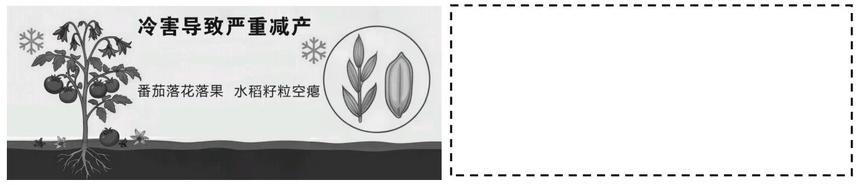
\includegraphics[width=11cm]{q4-duizhaotu.png}
\end{center}

\par\vspace{2.2em}

\question{5}{学校记者团获得了采访许操的机会，将面向全体同学，在校刊《晨光》上推出一篇深度人物访谈。他们研读了阅读I的三则材料，并准备了一些采访问题。记者团比较认可以下三个问题，请你提炼它们的共同特点，并据此为记者团再补充一个采访问题。（6分）}

\par\vspace{0.2em}
\noindent\hspace{2em}问题一：在实验室中取得的关于RGF的成果，应用到真实农田中，可能会出现哪些意料之外的情况？\par
\noindent\hspace{2em}问题二：八年科研攻关，您和团队经历的最困难的事情是什么？有没有想要放弃的时候？\par
\noindent\hspace{2em}问题三：您对学生娄焕昌的安慰幽默又暖心，您希望年轻人从“失败”中学到什么？\par

\par\vspace{2.2em}

\subsechead{（二）阅读II（本题共4小题，18分）}
阅读下面的文字，完成6～9题。

\begin{center}{\bfseries 最后的鼓王}\par\vspace{0.15em}陈文双\end{center}

\begin{materialtext}
在莫索镇，最早醒来的是炊烟，它们醒来之后，再继续摇醒大地上的其他事物。炊烟升到一定高度，会跟晨雾和水汽搅和在一起，平铺着，在半空中形成一层松散、平行而又很有条理的烟岚。晨风徐来，那层烟袅袅娜娜，出现小幅度的扭曲，像松树木头的切面。其实，它更像一幅画，一幅上面铺着一层厚厚丝绸的画。

罗小民穿过小镇，朝校门口走去，他发现街道两边出现了很多鲜红的宣传标语——热烈庆祝南安县鼓书大王擂台赛在我镇举行。这是本镇有史以来最大的文艺盛事，怠慢不得。

爷爷昨天一定是到镇里报名去了，所以连鸭子都可以不管。可是，他很替爷爷担心，爷爷曾向奶奶发过誓，再也不去当打鼓匠。

爷爷罗一木出身鼓书世家，鼓书技艺传到他手上不知道是多少代了，他的名号凡是澧水下游，跑过点江湖的可谓无人不知，无人不晓。罗一木的父亲，艺名罗天响，曾是莫索河上的一代鼓王。四九年解放军南下，从此过境，罗天响带着儿子在老码头为解放军专门表演节目，只有十来岁的罗一木在那次演出中一炮而红，当时还上过报呢。罗一木的儿子罗树林，能接他的班，对鼓、三棒鼓、渔鼓，样样精通。

这都是二十年前的事了，作为孙子，罗小民也是从别处听来的。爷爷说，将来要让罗小民接班，把祖辈的技艺传下去。罗小民不学，他怕同村的孩子编话骂他，“龙生龙凤生凤，鼓匠的崽崽闹丧场”，死了人，鼓匠必须去唱，唱得越大声越好，这就叫闹丧。其实，这打鼓啊，据说是庄子他老人家发明的，有一天，庄子的老婆死了，他拿着个脸盆在灵前拍着唱，旁边的人觉得脸盆不雅观，不好看，就给他换了个鼓，如此，传到了现今……

罗小民问爷爷：“真的要去唱？”

“当然去，鼓王奖金有四千块，放鸭子要放一年。”

“奶奶那怎么办？”

“你不说，我不说，她怎么知道？”

爷爷看着孙子，双眉紧蹙不说话。孙子早就读出了爷爷的心思。

莫索河静静流淌，没日没夜，它经历了繁华，也经历了萧条，并没因为老码头上有船停靠或者没船停靠，而变得干涸，好像这个世界与它没有多大关系，住在它边上的人有着怎么样的烦恼也跟它没有什么关系，它只是流，日夜不息。

爷爷每天按时去放鸭，到天黑了也按时回来。只是，这个按时之中添加了别的东西，爷爷在偷偷创作新的鼓词，抄好了塞在衣袖里，没人的时候，就拿出来背。

那天，罗一木起得很早，打算提前半小时将鸭子赶出去。鸭子快把谷子吃完时，罗一木转身进屋，穿上前日新浆洗的衣服，等他再次跨出门槛的时候，身后传来一阵响动。

“放鸭子还穿新衣服？你要想打鼓，除非等我死了！”

罗一木回头，看见老太婆，唯诺道：“最后一回，四千块……”

“男人说话，巫婆打卦，要字字作数。”

罗一木不说了。

他退回屋里，将新衣服脱下，这时他看见（\blank[5em]）。他戴了草帽，赶着鸭子出了门，那个背影缓缓走向田野深处，在天空下显得那么孤单与落寞。

星期六，老码头庆丰茶楼的老板王金宝对罗小民说，告诉你爷爷，就说老伙计要他到茶楼来一趟。

罗一木去了才知道，县文化馆下来一个文学专干小陈，要找他。县里决定将这个地区的鼓书艺术申请非物质文化遗产名录，首先要从最具传承说服力的老艺人入手，小陈说得很动情，也很真诚，可罗一木不觉得这件事与自己有什么关系。

这时，王金宝说：“茶楼已经转给刘老板当游戏厅，过几天就搬，你不来，以后就没有机会了，最后一场，茶楼从此关门。”

不知从什么时候开始，小镇上也有了卡拉ok，有了美容院，茶馆的生意自然就清淡下来。

最后一场。茶楼过几天就没有了。这些话像钉子一样扎疼了罗一木的心，他在这里打了几十年鼓，如今，说没就没了？

罗一木咬了咬牙：“好，就明天，老婆子那里得瞒过去。”

茶馆里空空荡荡，那些桌椅板凳都旧了，王金宝早上起来擦了半天，还是不亮，房顶上的那两片亮瓦也太久没有清理，长了一层厚厚的苔藓。王金宝看着这些东西，突然生出一种陌生感，他就在这里干了几十年？他抬头看了看那两块模糊不清的亮瓦，越看越不顺眼，后来，干脆架楼梯上去，将它们捅碎了，两块亮瓦掉在地上摔得稀烂，屋顶成了两个透明的窟窿，光毫无阻隔地照到了前台。

台上架着一面鼓，鼓上安静地卧着两根木棍，木棍和鼓在等待它们的主人，那个久违了的主人。

没人广播，但镇上的人似乎都知道了老罗要出山的消息，他要到庆丰茶楼打鼓，打最后一场鼓！该来的都来了，没有一个空位子，仿若旧时盛况，这些过去的铁杆鼓迷都老了。

看到这么多熟人，罗一木很有些感动，眼睛一下湿润起来，脚步也有些迟缓，他迈着那两条跟着他经历了七十年风霜雪雨的老寒腿，徐步走向前台。

“秦琼卖马，子胥吹箫，自古英雄，也曾困乏。话说，秦叔宝走到潞州……”

刚起腔，罗一木便抬头看见老太婆站在了茶馆的门口，他吐到嘴边的唱词又咽了回去。大家睁大眼睛齐刷刷看着他，然后，又扭过头去看老太婆。

茶馆一片死寂。

鼓没打成，奶奶也病了。

现在，罗一木再也不用担心谁来反对了，他要出门打鼓，捞钱给老婆子当医药费，为孙子凑学费。他打定主意，就走以前走过的那条路线，一个村一个村的去，一个院一个院子的去，穿街走巷，上门去唱。没有了茶馆，他只好回到最原始的阶段，上门不适合打双棍大鼓，只能捧着竹筒唱渔鼓。

就在他去外面打渔鼓的时候，老婆子一个人走了。罗一木很后悔，连老婆子最后一面都没见着，没能送她最后一程。

黄昏时分，罗一木又敲起了鼓，这一次，他敲得专注而用心，最后连眼睛也闭上了，他进入了忘我的状态，入神了。观众也跟着入神了。人人都知道罗一木的鼓打得好，但从未听过如此精湛的表演。越来越多的人围了过来，他们听了很久，才想起来问：“怎么？你奶奶又准他打鼓了？”

“奶奶死了。”

“啊？死了？”

孙子与外人的对话，罗一木一句没听见，他只是打他的鼓——

\begin{center}
小孩没得娘，说来话就长。\\
好男不种爷家田，\\
六月冻死老绵羊。\\
三百六十行，\\
偏学做鼓匠，\\
世代来相传，\\
到我不像样，\\
时也命也哉，\\
谁能说清白，\\
哎嗨哟，谁能那个说清白……
\end{center}

待人们走近细看，发现罗一木脸上已是老泪纵横。

夜色中，人们只看见他脸上的泪，看不清表情如何。人们都说，老罗对自己女人好，那堂鼓打得肺腑皆空，在场的人无不动容。\uline{直到第二天早上人们才明白，那鼓其实是他为自己敲的。}
\end{materialtext}
\begin{flushright}（有删改）\end{flushright}

\question{6}{下列对文本相关内容和艺术特色的分析鉴赏，不正确的一项是（3分）}
\begin{choices}
\item “晨风徐来，那层烟袅袅娜娜……一幅上面铺着一层厚厚丝绸的画”，写出了小镇清晨的宁静，也为后文表现传统艺术的衰落营造了氛围。
\item 奶奶识破了罗一木想要登台打鼓的心思，“男人说话，巫婆打卦，要字字作数”这处语言描写，塑造出奶奶刻薄、执拗、不近人情的形象。
\item 莫索河“静静流淌，没日没夜……它只是流，日夜不息”，见证了罗一木一家的烦恼，也以自己的恒常不变反衬出人世变迁。
\item 王金宝捅碎亮瓦，主动打破传统的茶馆空间，让光“毫无阻隔地照到了前台”，这一细节具有象征意味，暗示着他将与过往生活告别。
\end{choices}

\question{7}{根据你对文本的理解，在文中括号处补写一段景物描写，要求能够表现罗一木放弃参加擂台赛后的心理，衔接自然，字数在60～90字之间。（5分）}

\par\vspace{2.2em}

\question{8}{阅读本文时，有读者读出了亲近，有读者读出了疏离。哪一种更贴合你的阅读体验？请从叙述艺术的角度说明理由。（4分）}

\par\vspace{2.2em}

\question{9}{有人觉得小说最后一句话可以删去，请谈谈你的理解。（6分）}

\par\vspace{2.2em}

\subsechead{（三）阅读III（本题共5小题，23分）}
阅读下面的文言文，完成10～14题。

\material{材料一：}
\begin{materialtext}
臣\zd{伏}以史者，国家之典法也。自君臣善恶功过与其百事之废置，可以垂劝戒示后世者，皆得直书而不隐。故自前世有国者，莫不以史职为重。伏见国朝之史，以宰相监修、学士修撰，又以两府之臣撰时政记。选三馆之士当升擢者，乃命修起居注。如此，不为不重矣。然近年以来，员具而职废。其所撰述，\zd{简}略遗漏，百不存一，至于事关大体者，皆没而不书。此实史官之罪，而臣之责也。
\end{materialtext}
\begin{flushright}（节选自欧阳修《论史馆日历奏》）\end{flushright}

\material{材料二：}
\begin{materialtext}
孔子作《春秋》，盖曰其事则齐桓、晋文，其文则史，其义则孔子自谓有取乎尔。夫事即后世考据家之所尚也，文即后世词章家之所重也，然夫子所取，不在彼而在此，则史家著述之道，岂可不求义意所归乎？自迁、固而后，史家既无别识心裁，所求者\zd{徒}在其事其文。

\uline{惟郑樵稍有志乎求义，而缀学之徒，嚣然起而争之。}然则充其所论，即一切科举之文词，胥吏之簿籍，其明白无疵，确实有据，转觉贤于迁、固远矣。
\end{materialtext}
\begin{flushright}（节选自章学诚《文史通义·内篇五·申郑》）\end{flushright}

\material{材料三：}
\begin{materialtext}
春秋大义，\zd{诛}乱臣贼子，人人所知，而前人之论过于宽纵，后人之论过于苛刻，皆未合春秋之旨。

谓前人之论过于宽纵者，左氏采各国旧史以成文，当时邪说杂在其内。杜预解传，更扬其波。杜预专阿左氏，孔疏偏袒杜注，与春秋诛乱贼之旨，大相刺谬，所谓过于宽纵者此也。

谓后人之论过于苛刻者，春秋书晋赵盾弑其君夷皋，许世子止弑其君买，乃责备贤者之义，谷梁云因其自责而责之，是也。欧阳修谓赵盾弑君\xq{1}，必不止不讨贼；许止弑君\xq{2}，必不止不尝药，以三传皆不足信。夫从三传之说，未尝不可严名教之防。盾既书弑君而复见其名，止既书弑君而又赦其罪，正可见圣人执法虽严，而待人甚恕。谷梁曰：“\wave{于盾也见忠臣之至于许世子止见孝子之至}。”事非目睹，何必翻前人成案，使与亲弑者同科乎？\uline{欲申春秋诛乱贼之旨，而不得其平，所谓过于苛刻者此也。}
\end{materialtext}
\begin{flushright}（节选自皮锡瑞《师伏堂春秋讲义》）\end{flushright}

[注]\xq{1}赵盾弑君：晋灵公无道，赵盾族弟赵穿弑君。赵盾身为正卿未诛赵穿，太史董狐书“赵盾弑其君”。\xq{2}许止弑君：许止，许悼公之子，《左传》载其因进药不当致父死，非亲手弑君。

\question{10}{材料三画波浪线的部分有三处需要断句，请用铅笔将答题卡上相应位置的答案标号涂黑。（3分）}

\duanju{于盾也A见忠B臣之C至D于E许世子F止G见H孝子之至}

\question{11}{下列对材料中加点的词语及相关内容的解说，不正确的一项是（3分）}
\begin{choices}
\item “伏”，敬词，与《陈情表》中“伏惟圣朝以孝治天下”的“伏”用法相同。
\item “简”，简略、简省，与《谏太宗十思疏》中“简能而任之”的“简”用法不同。
\item “徒”，只是、仅仅，与《孔雀东南飞》中“徒留无所施”的“徒”意思不同。
\item “诛”，谴责、责问，与《六国论》中“洎牧以谗诛”的“诛”意思、用法相同。
\end{choices}

\question{12}{下列对材料有关内容的概述，不正确的一项是（3分）}
\begin{choices}
\item 欧阳修认为，历代君主无不重视史官，但近年来史书的撰述却存在缺漏，那些关乎国家根本的大事未被记载，对此史官是有责任的。
\item 若史家仅关注事与文，那么科举文词、胥吏簿籍清晰无误，记事确凿，其价值远高于司马迁、班固的史书，章学诚认为这是错误的。
\item 《左传》采择各国旧史撰写成书，杜预在为其作注解时，在原文中混入并宣扬了当时的一些邪说，使得它们的影响进一步扩大。
\item 欧阳修对《春秋》三传的记载有所怀疑，认为赵盾和许止的行为如被定性为“弑君”，其罪行绝不止“不讨贼”或“不尝药”。
\end{choices}

\question{13}{把材料中画横线的句子翻译成现代汉语。（8分）}

（1）惟郑樵稍有志乎求义，而缀学之徒，嚣然起而争之。

（2）欲申春秋诛乱贼之旨，而不得其平，所谓过于苛刻者此也。

\question{14}{请依据三则材料中体现的评述历史的不同原则，简要评析贾谊的《过秦论》或苏洵的《六国论》（150字以内）。（6分）}

\par\vspace{2.2em}

\subsechead{（四）阅读IV（本题共3小题，15分）}
阅读下面两首宋诗，完成15～17题。

\begin{center}{\bfseries 重送祖择之北使}\par\vspace{0.15em}梅尧臣\end{center}

\begin{poem}
文章世德已能传，得桂高枝二十年。\\
持节欲同苏武劲，下帷曾似董君贤。\\
衣裘衽领无嫌左，饮食杯盂暂厌膻。\\
一过范阳\xq{1}应感慨，归来图画彼山川。
\end{poem}

\begin{center}{\bfseries 至济南李公择以诗相迎次其韵二首（其一）}\par\vspace{0.15em}苏轼\end{center}

\begin{poem}
敝裘羸马古河滨，野阔天低糁玉尘。\\
自笑餐毡典属国\xq{2}，来看换酒谪仙人。\\
宦游到处身如寄，农事何时手自亲。\\
剩作新诗与君和，莫因风雨废鸣晨。
\end{poem}

[注]\xq{1}范阳：地处宋辽交界，宋时属辽国。\xq{2}典属国：苏武曾被任命为典属国，此处以官职代人。

\question{15}{下列对这首诗的理解和赏析，不正确的一项是（3分）}
\begin{choices}
\item 祖择之家学深厚，科举登第已有二十年，诗人从家世、仕途两方面对友人予以称誉。
\item 诗人料想友人途经范阳会心生感慨，并劝勉其归来后绘录北国山川，期许其能不辱使命。
\item “敝裘羸马古河滨”通过列锦的方式，勾勒羁旅困顿的画面，营造苍凉萧索的氛围。
\item 苏诗颈联写出了诗人因宦游四方、辗转奔波而心生厌倦，相信终有一日能辞官归田。
\end{choices}

\question{16}{用典贵在贴切，诗人可截取典故的不同侧面以寄情志，请结合“持节欲同苏武劲”“自笑餐毡典属国”两句简要分析。（6分）}

\par\vspace{2.2em}

\question{17}{补写出下列句子中的空缺部分。（6分）}

（1）《梦游天姥吟留别》中的“\blank[6.5em]，\blank[6.5em]”两句，最能体现“谪仙人”李白蔑视权贵、傲岸不屈的品格。

（2）班会课上，同学们坦言追梦之路并不容易。马老师写下了《论语·泰伯》中的“\blank[6.5em]，\blank[6.5em]”两句，借此鼓励大家树立远大抱负，锤炼坚韧品格，不惧艰难险阻。

（3）古代诗文中，表现奉献精神的句子层出不穷，比如：“\blank[6.5em]，\blank[6.5em]。”

\sechead{二、语言文字运用（本题共4小题，15分）}
阅读下面的文字，完成18～21题。

{\ywkai 在叙事的时候，一端未了，以另一端直起突接，转叙他事，虽感突兀，却能跳脱冗杂和庸俗，这种修辞格叫做“突接”。突接与“顶真”恰好相反，“顶真”是抱紧上句的字词，直线连下，突接是要和上句绝不相关，劈空而来的。

如《史记》鸿门之宴中樊哙答项王的话：“臣死且不避，卮酒安足辞！夫秦王有虎狼之心，杀人如不能举，刑人如恐不胜……”在“卮酒安足辞”句下，突接一段议论，“夫秦王……”根本与上文不相关，虽然“死且不避”四字，可以暗与下面“沛公先破秦”“劳苦而功高如此”等话引接，终究不合语言的连贯性。但依当时的情势来看，实在也不容迁缓地道出，这样一用突接，非仅可以体味当时（\blank[3em]）的情势，而壮士瞠目的神情也跃然纸上，同时语势也不会迂弱了。

在诗中，意外的宽对，会造成张力，而意义相似的“合掌对”反而疲软复沓，这道理与突接的修辞原理相同。如宋代方夔的《杂兴》诗：“鸟不惊猜无忤物，人多怒骂渐逃名！”上下两句，毫不相干。上句似用庄子海鸥不相猜疑事，下句则说人到了喜欢愤世怒骂的时候，大概也不想成名立业了！两句一经突接，像规劝，像自责，像不受世故的沾染，像不顾社交的规范，许多意思凑集在里面，两句之间的承接说明，全省脱在言外了。

再则如诗中的集句集联，没来由的忽然将两个无涉的旧句，牵合成对，产生出陌生而全新的喜悦，也与突接的修辞原理相类似。像“红杏枝头春意闹”的名句，无端与唐诗“乌衣巷口夕阳斜”凑合，新意涌出，别成丽景。又如将“劝君更尽一杯酒”的口头熟句，无端与李白诗“与尔同销万古愁”凑合，辞意顺溜，工稳绝妙。又如将杜牧的“古往今来只如此”与苏轼的“淡妆浓抹总相宜”凑合，挂在舞台两侧，将戏剧与人生总括在一起，大出原句意外，胜于一切雕巧了。\par}

\question{18}{填入文中括号内的词语，最恰当的一项是（3分）}
\begin{choices}
\item 同室操戈
\item 枕戈待旦
\item 剑拔弩张
\item 如临深渊
\end{choices}

\question{19}{关于材料第三段的理解与分析，以下正确的一项是（3分）}
\begin{choices}
\item “意外的宽对，会造成张力”，使用逗号形成停顿，突出了陈述对象，但也使文意不流畅。
\item 文段以宋代方夔《杂兴》中的诗句为例，论证意外的宽对能产生文学张力，这是以偏概全的表现。
\item “大概也不想成名立业了”中，“大概”一词表明这是作者的主观推测，影响了整体语段的严谨性。
\item 尾句中连用四个“像”，以铺陈的方式，表现了妙用突接所生发的多重审美联想，富有韵味。
\end{choices}

\question{20}{根据上下文语境，完成下列两个小题。（6分）}

（1）梳理“合”字义项，补全表格A、B、C处。（3分）

\xq{1}不合　\xq{2}合掌对　\xq{3}牵合　\xq{4}凑合

\begin{center}
\setlength{\tabcolsep}{4pt}
\begin{tabular}{|c|l|}
\hline
序号 & 义项 \\
\hline
A & 符合 \\
\hline
\xq{2} & B \\
\hline
C & 凑到一起 \\
\hline
\end{tabular}
\end{center}

（2）按照词义引申的一般规律，为上表中的义项排序。（3分）

\blank[4.5em]$\rightarrow$\blank[4.5em]$\rightarrow$\blank[4.5em]

\question{21}{从你学过的古诗文中任选两句，运用“突接”，仿照示例，设计一则以“修身”为主题的座右铭，并简要说明衔接成立的理由。（3分）}

示例一：少年辛苦终身事，柳暗花明又一村。

示例二：居高声自远，只留清气满乾坤。

\sechead{三、写作（60分）}

\question{22}{阅读下面的材料，根据要求写作。（60分）}

{\ywkai 阅读I材料二描述了许操团队将灵感转化为成果的过程，向我们展现出了一条探索世界、认识世界的路径：由观察引发猜想，由猜想带来新的发现。}

以上材料引发了你怎样的联想和思考？请写一篇文章。

要求：选准角度，确定立意，明确文体，自拟标题；不要套作，不得抄袭；不得泄露个人信息；不少于800字。

\end{document}
